\chapter{Lecture Review}

    We first introduce building blocks of our model, consisting Support Vector Machine(SVM), Multi-layer Peceptron
(MLP), Random Forest, Restricted Boltzmann Machine (RBM), Conditional Restricted Boltzmann Machine, and Hyper Model. A brief overview of these models, we can divide these models in to two categories, supervised learning and unsupervised learning. Supervised learning is just like how teachers and dear supervisors teach us, giving us some examples, which are "labeled" by them, and we learn from the examples, however unsupervised learning is teachers give us a criteria to identify different objects, and we use the criteria to learn.



\section{A brief theoretical look into Machine Learning}
    A general issue Machine Learning models want to resolve is how well we can approximate the true generative function $f:\mathbf{X}\rightarrow\mathbf{Y} $, which generates observable data.
   
    For instance, as an economist, we are interested in forecasting future GDP, or other economic indices. Assume that $GDP_{t+1} =f(C_{t})$ is the truth, and we want to use our algorithm to choose $g(x)$ to approximate our target function $f(x)$, given the data $(\mathbf{x_{n}},\mathbf{y_{n}}) $ generated by the target function $f(x)$.% general model setup
%place the image

When we have the general setup of machine learning models, % what's model learned? how we get g(x)


Since we got the optimal $g(x)$ from our hypothesis set$\mathbf{H}$, how we assessment whether we have 'learned' from the data, or we just memorizing the labels in our data set.% how we evaluate the model

\clearpage
\subsection*{Model Complexity}
\subsubsection*{VC dimension}
Now we introduce the concept of VC dimension.
VC dimension (for Vapnik Chervonenkis dimension) (Vapnik and Chervonenkis (1968, 1971), Vapnik (1979)) measures the capacity of a hypothesis space. Capacity is a measure of complexity and measures the expressive power, richness or flexibility of a set of functions by assessing how wiggly its members can be.

\begin{defn}
The Vapnik-Chervonenkis dimension of a hypothesis set $\mathbf{}{H}$, denoted by $d_{vc}(\mathbf{H})$ or simply $d_{vc}$, is the largest value of $\mathbf{N}$ for which $\mathbf{m_{\mathbf{H}}}(\mathbf{f(N)})= 2^{N}$. for all $\mathbf{N}$ then $d_{vc}=\infty$

\end{defn}
%
For example, assume $\mathbf{H}$ is a hypothesis set which is linear separation model(use a line to separate data), we are given pairs of ${x_{n}, y_{n}} $, and $ x_{n} \in \mathbf{R^2}$. How many different binary combinations can we assign to the data set?

\begin{center}
{
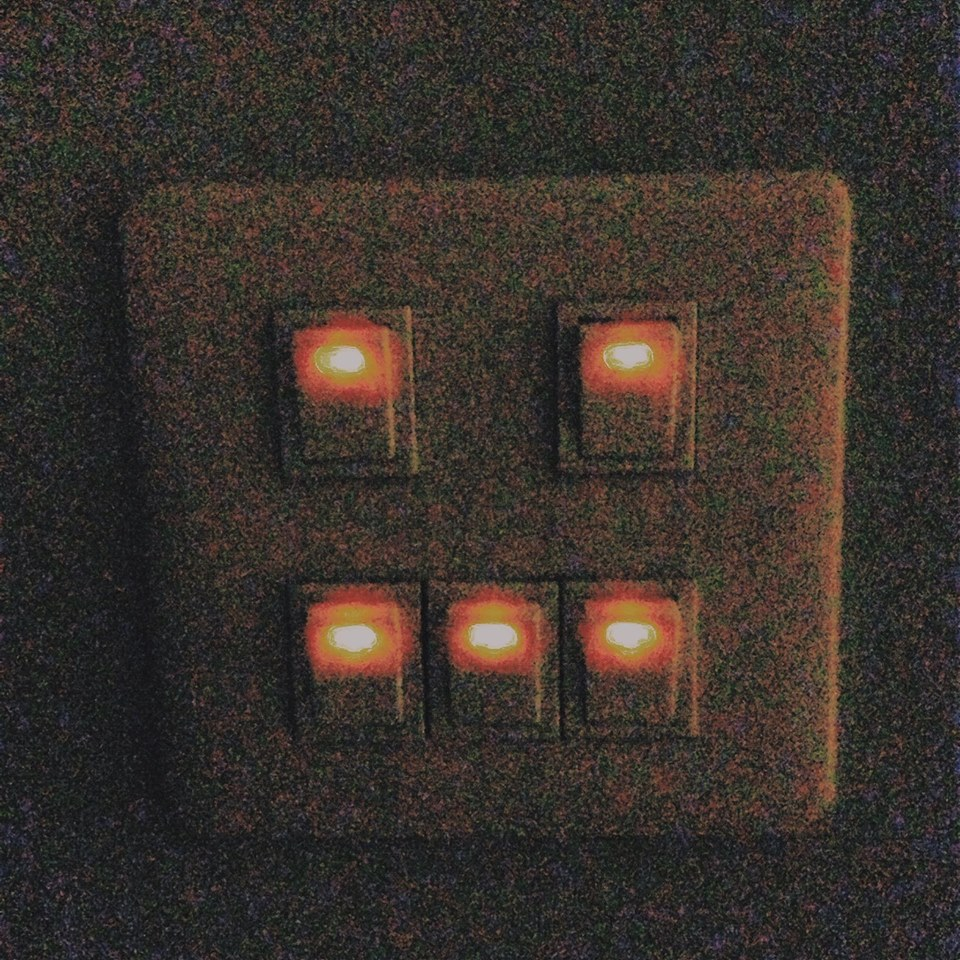
\includegraphics[width=7cm]{OOO}
}
\end{center}

%----- end VC dimension
\subsection*{Penalty for Model complexity}
Now we fuse above concepts together explaining the core philosophy of our modeling process.
%----what is E_out ? E_val?
As our model complexity increasing, the less in sample error we will get, however we would probably get a very high error out of sample. This issue is called over-fitting. Over-fitting is everywhere, anytime.  Every steps in our modeling process would be leading us to the trap of over-fitting, for instance our past experience, belief, even knowledge.
In general method to prevent this deadly trap, we employ the out of sample error. We divide our observable sample data into two group a test set, and a learning set, further more we split the learning set into validation set and training set. 
%As we have assigned the different sets from different purposes we can plot what we call a learning curve.

\subsection*{Cross Validation\& Model Selection}
There are plenty of methods, and criteria delicate themselves on model selection. In a very general and robust approach, we use cross validation as our method to select model.

\section{Supervised Learning}

\subsection{Support Vector Machine}

Cortes and Vapnik, Support Vector Machine(1995) is a discriminative model. We can write our problem into a general form.
$$ y = g(\sum^{K}_{i=1}{x_{i}}) \quad \textrm{and} \quad K \in \mathbf{R}$$
For basic model, $y \in \{-1, +1\}$  and $\ x_{i} \in \mathbf{R^{K}}$.
The formula shows SVMs can be easily applied on the regression model which we are familiar with. To introduce SVM we first introduce Hard-Margin Support Vector Machine(HmSVM).
\clearpage

The model can be written informally as follow.

$$\large{\max_{\mathbf{W}}} \ margin(\mathbf{W})$$
$$ s.t\ margin(\mathbf{W})=\min_{n=1...N} Distance(\mathbf{x_{n}},\mathbf{W})$$
$$ and\ \forall \ n \ y_{i}(\mathbf{W}^{T} x_{n})>0$$
The maximization problem is to find the 'fattest' tube to perfectly separate our data, assuming the data set is separable(so called hard margin).
More clearly to illustrate SVM is to use graph, we have a data set which is already labeled in +1, and -1, ploted below.\\

\begin{center}
{
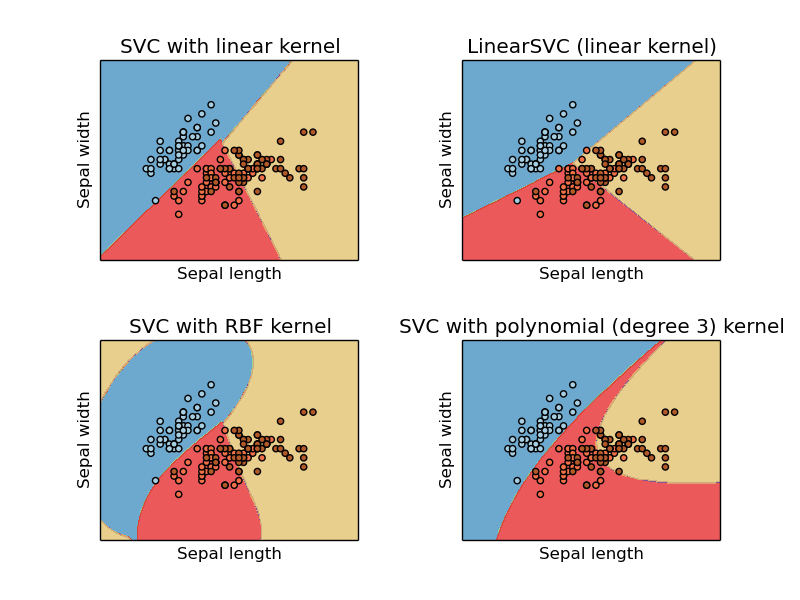
\includegraphics[width=10cm]{SVM.png}
}
\end{center}
The solution of hard-margin SVM is the red-colored tube which is the "fattest" from all potential candidates which can classify all training data.

As you can see from (1), hard-margin SVM does not assume any underlying distribution of our data set, but only the assumption of separability of our data set. However this condition can be easily loose by putting an bias term $\zeta$ 

%\subsubsection{Prime Problem}
%More formal form of hard margin SVM is to rewrite the problem into quadratic form.

%\subsubsection{Dual Problem}

%More formal form of hard margin SVM is to rewrite the problem into quadratic form.

\subsubsection*{Kernel Transformation}
More formal form of hard margin SVM is to rewrite the problem into quadratic form. 
\subsubsection*{Poly Nominal Kernel}

\subsubsection*{Radial Basis Function Kernel}

%\subsubsection*{Support Vectors}
%Sparse solution


\subsection{Multi-layer Perceptron}

\subsubsection*{L1 and L2 regularization}

\subsection{Random Forest}

\subsubsection{Decision Tree}

\subsubsection*{Bagging}

\subsubsection*{Model Selection}

\subsection{Conditional Boltzmann Machine}

\subsubsection{Autoencoder}
Now we introduce the concept of autoencoder

\subsubsection{Historical Effect}

    For general time series technique is that putting lag-terms in each sample, in the form of auto-correlation regression($AR(p)$).
    
    This method is very expensive when we facing high dimensional data, not only cost us to abandon the degree of freedom but also make our validation and testing procedure very time consuming.
    
    On the good side of this method is that it do not need any adjustment of the transformation process, just put the lag-terms in the data.
    
    Another approach is to use the Conditional Restricted Boltzmann Machine(CRBM). CRBM can server as an autoencoder of the training data set, unlike PCA does not take past pattern into consideration, catch the historical unique pattern into the generation process.